\runningheader{Oppgave f)}{}{Side \thepage\ av \numpages}

\item[]   Alle modellene i denne delen av øvingen skal implementeres
  i subsystemet\\
  \fbox{\tt Om Sine Wave-blokken, oppgave 2f)-2h)} i 
  skallfilen \fbox{\tt oving2.slx}.



% ********************************************************
% oppgave f) 
% ********************************************************  
\item
  I denne oppgaven skal du implementere signalet $u(t)$
  \begin{equation}
    \label{eq:208}
    u(t) = 3.2\sin(1.2t)+2
  \end{equation}
  på 2 måter som vist i figuren under. Ved å sammenligne kurvene i
  scopet vil du kunne se at de gir samme resulatet.
  \begin{figure}[H]
    \centering
    \hspace*{0mm}\scalebox{1.2}{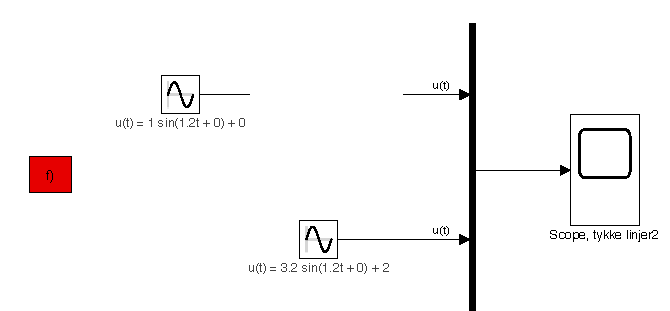
\includegraphics{2f.pdf}}
  \end{figure}

  \begin{itemize}
  \item 
  Den øverste varianten tar utgangspunkt i en 
  {\sf  Sine Wave}-blokk som kun gir ut
  \fbox{$\sin(1.2t)$} med amplitude lik 1 og ingen likevektsverdi (bias).
  Det betyr at du må bygge opp signalet $u(t)$ ved å bruke et utvalg
  av andre blokker, som {\sf  Gain}, {\sf  Constant} og {\sf 
    Sum}. Det er flere måter å gjøre dette på, og detaljene om dette
  er skjult i modellen under. 

\item  Den nederste varianten er  en  {\sf  Sine Wave}-blokk hvor
  amplituden og likevektsverdien til $u(t)$ er spesifisert direkte i blokken.
  \end{itemize}

  {\color{red}La simuleringstiden fortsatt være 25 sekund.  }

      {\bf Gjør følgende oppgaver / svar på følgende spørsmål:    }
  \begin{enumerate}[label=f\arabic*)]
  \item   Bygg ferdig modellen og ta et skjermdump av modellen
    i innlevereringen  din.
    \item  Simuler modellen og ta med simuleringsresulatet
    i innleveringen din.
    For å vise at kurvene ligger over
  hverandre MÅ du endre den  røde kurven til å være  stiplet slik
  at det er mulig  å se at de ligger over hverandre.

  \item   Uttrykket for $u(t)$ i ligning~\eqref{eq:208} kan generelt skrives som
  \begin{equation}
    u(t) = U {\cdot} \sin(\omega{\cdot}t) + u_{A}
  \end{equation}
   Anta at du ikke kjenner til uttrykket for  $u(t)$, men bare har
   kjennskap til figuren med resultatet ditt.
   Vis hvordan du ved hjelp av \underline{kun avlesninger} fra kurven i scopet kan
   beregne estimater av følgende størrelser:
   \begin{itemize}
   \item amplituden  $U$
     \item frekvensen $\omega$ 
   \item likevektsverdien $u_{A}$
   \end{itemize}
   
  \end{enumerate}
